\documentclass[11pt]{beamer}

\usetheme{metropolis}

\usepackage{graphicx}
\usepackage{physics}
\usepackage{adjustbox}
\usepackage{caption}
\usepackage{chemformula}
\usepackage{quoting}
\usepackage[style=chem-angew,backend=bibtex]{biblatex}
\bibliography{references}
%
% Choose how your presentation looks.
%
% For more themes, color themes and font themes, see:
% http://deic.uab.es/~iblanes/beamer_gallery/index_by_theme.html
%
\mode<presentation>
{
  \usetheme{default}      % or try Darmstadt, Madrid, Warsaw, ...
  \usecolortheme{default} % or try albatross, beaver, crane, ...
  \usefonttheme{default}  % or try serif, structurebold, ...
  \setbeamertemplate{navigation symbols}{}
  \setbeamertemplate{caption}[numbered]
  \setbeamerfont{footnote}{size=\tiny}
} 

\usepackage[english]{babel}
\usepackage[utf8]{inputenc}
\graphicspath{{image/}}

\AtBeginSection[]{
\begin{frame}{Outline}
  \tableofcontents[currentsection]
\end{frame}
}

\title{Chapter 3: Chemical Compounds}
\institute{Chemistry Department, Cypress College}
\date{Sept 7, 2022}

\begin{document}

\begin{frame}
  \titlepage
\end{frame}

\begin{frame}{Class Announcements}
  \begin{itemize}
  \item Inputted grades for up to the quiz
  \item When uploading assignments, be certain that
    the file is in a readable format e.g. docx, png, jpeg,
    and pdf
  \item Everyone performed pretty well on the quiz; average
    4.1 and standard deviation 0.84
  \item This week only, any late assignments will not be
    penalized $50\%$; submit late assignments by the Sept 7th
    at 11:59pm
  \item Quiz #2 released this Thurs, Sept 9 at 11am due Mon,
    Sept 12 at 11am
    \item Homework #2 released this Fri, 
  \end{itemize}  
\end{frame}

\begin{frame}{Lecture and Lab Weekly Agenda}
  \textbf{Lab Section}

  \begin{itemize}
  \item Finish Exp 1 - Laboratory Techniques
  \item There is no need to cut glassware and fire
    polishing
  \item Be familiarize with evaporation and filtration
    techniques
  \item Submit the lab worksheet due Sept 14 at 11:59pm;
    $50\%$ late penalty 
  \end{itemize}

  \textbf{Lecture Section}

  \begin{itemize}
  \item Go over homework assignment; present your work
    for 1pt EC
  \item Review Ch 2 - Atoms, Ions, and the Periodic Table
  \item Begin lecture on Ch 3 - Chemical Compounds and
    Ch 8.1 - 8.2 - Types of Bonding
  \end{itemize}
\end{frame}

\section{Review: Chapter 2 Highlights}

\begin{frame}{Atoms and Ions}
  \begin{itemize}
  \item Conservation of mass and conservation of energy
  \item Anions (gain electron) and cations (lose electron)
  \item Made up of protons, neutrons, and electrons
  \end{itemize}
\end{frame}

\begin{frame}{J.J. Thompson's Plum Pudding Model}
  \centering
  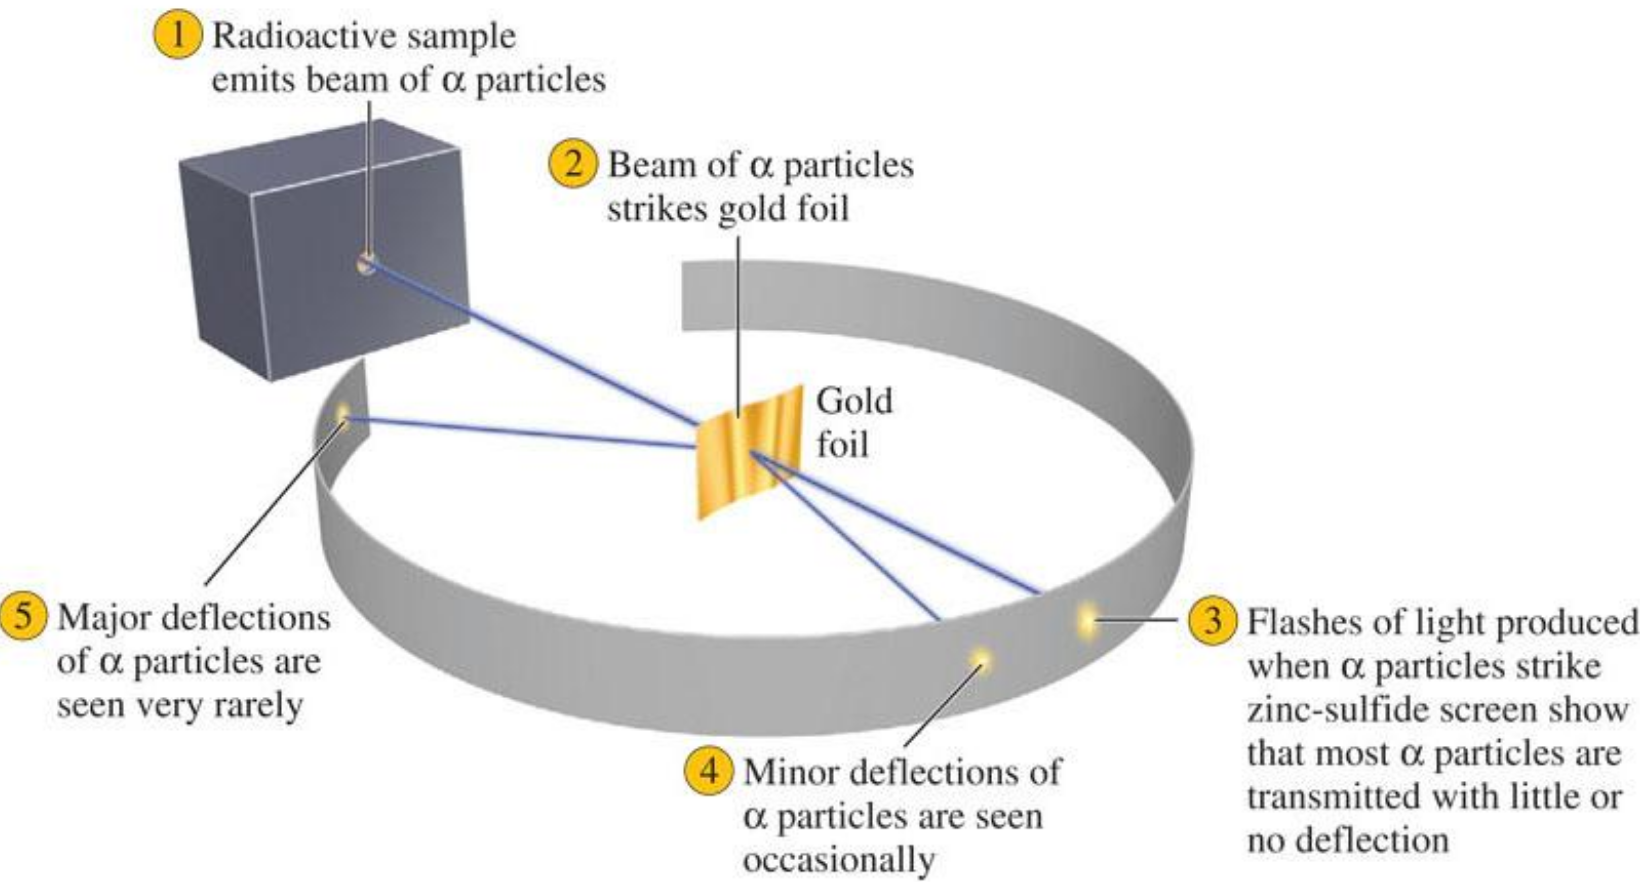
\includegraphics[scale=0.175]{alpha}
\end{frame}

\begin{frame}{Review: Modern Period Table}
  \centering
  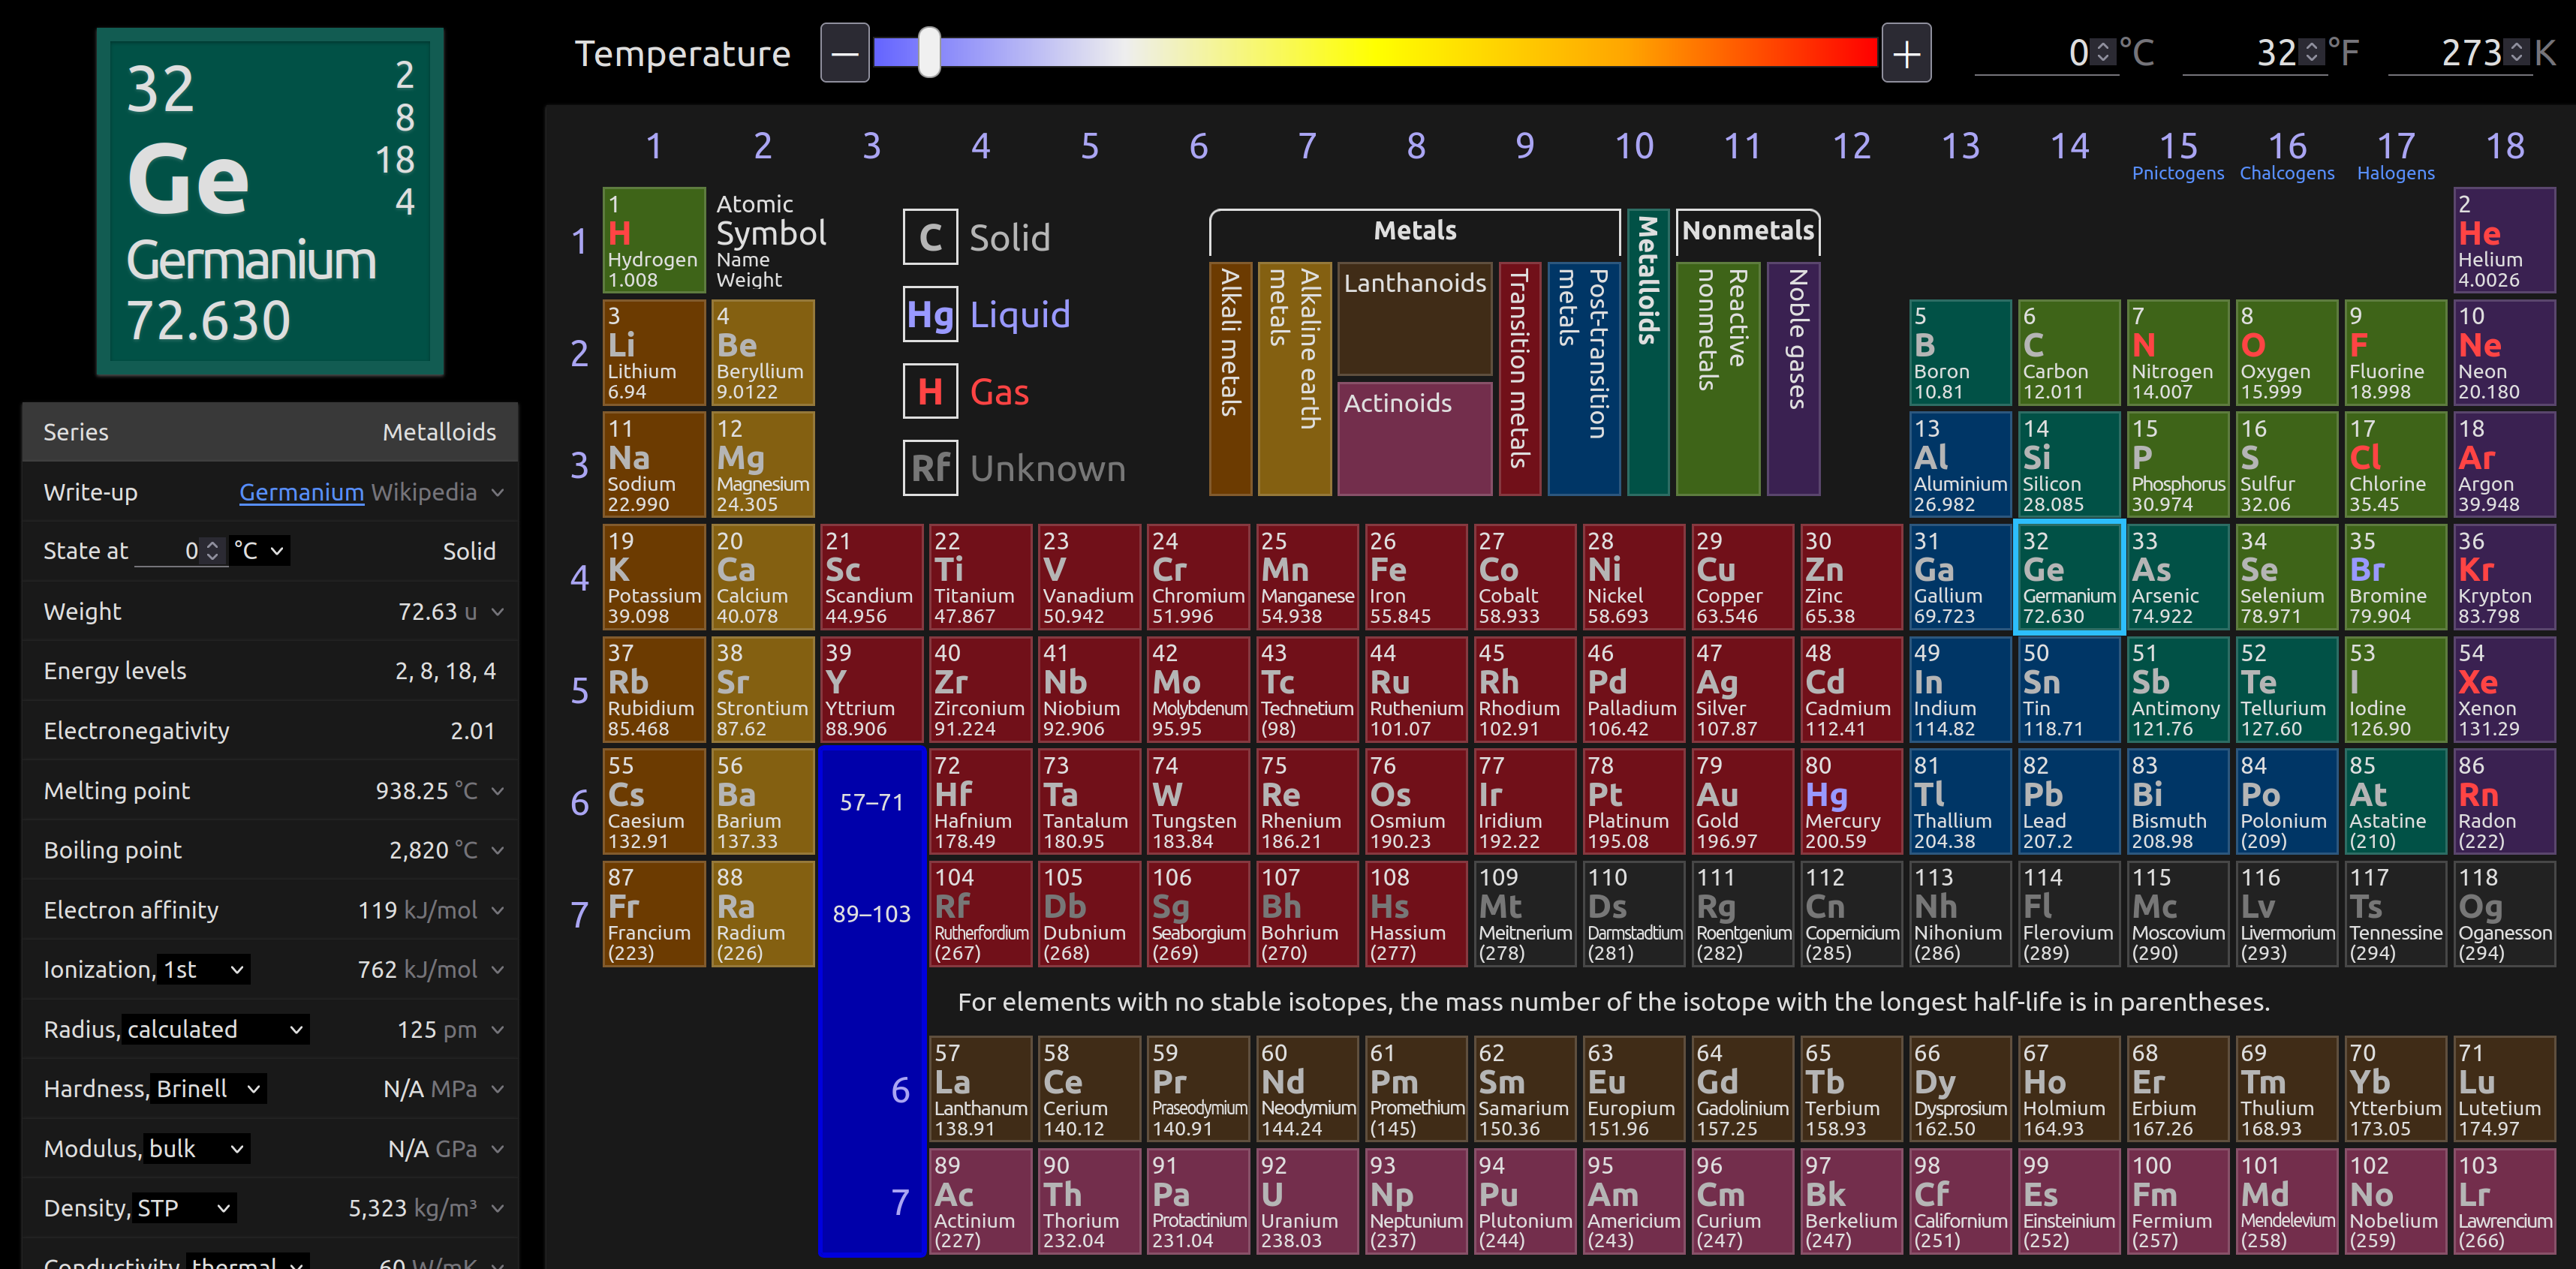
\includegraphics[width=\linewidth]{ptable}
\end{frame}

\begin{frame}{Relative Atomic Mass}
  \begin{equation}
    \text{Relative Atomic Mass} = (I_1\times A_1) + (I_2\times A_2) + \dots
  \end{equation}
  where $I$ is the mass of the isotope, and $A$ is the
  relative abundance between 0 and 1
\end{frame}

\begin{frame}{Defining Atomic Number and Mass}
  \begin{equation}
    ^\text{A}_\text{Z}\text{X}^\text{C}
  \end{equation}

  where A is the atomic mass, Z is the atomic number, X is atomic
  symbol, and C is the overall charge

  \textbf{Isotopes} - chemically same atom (same number of protons)
  but physically different (different number of neutrons)
\end{frame}

\begin{frame}{Hydrogen Isotopes and Applications}
  \begin{center}
    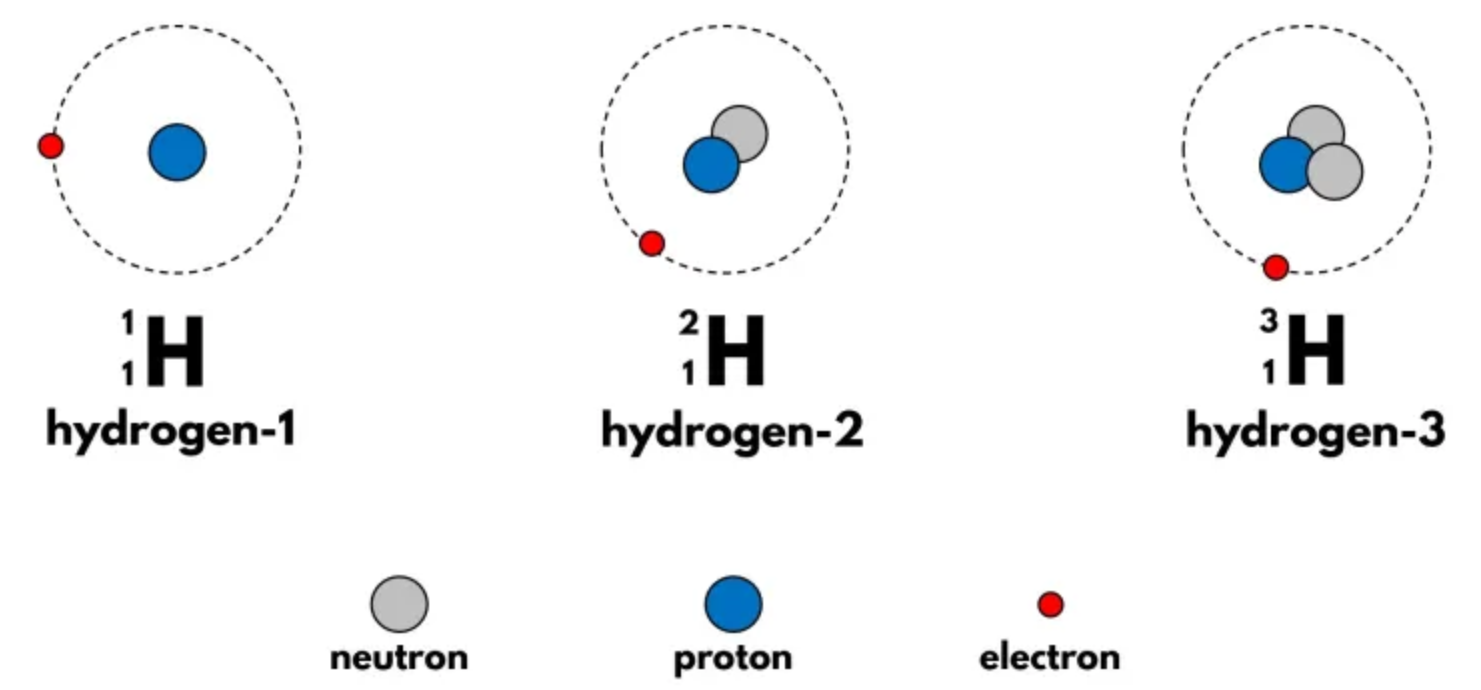
\includegraphics[width=0.75\linewidth]{hydro_iso}
  \end{center}

  \begin{itemize}
  \item Hydrogen ($^1_1$H), deuterium ($^2_1$D), and tritium ($^3_1$T)
    %have relative abundances of $99.84\%$, $0.0156\%$, and trace amounts,
    %respectively
  \item \textbf{Q:} Which hydrogen isostope is the highest in abundance?
  \end{itemize}
\end{frame}

\begin{frame}{Hydrogen Isostopes and Applications}
  \begin{center}
    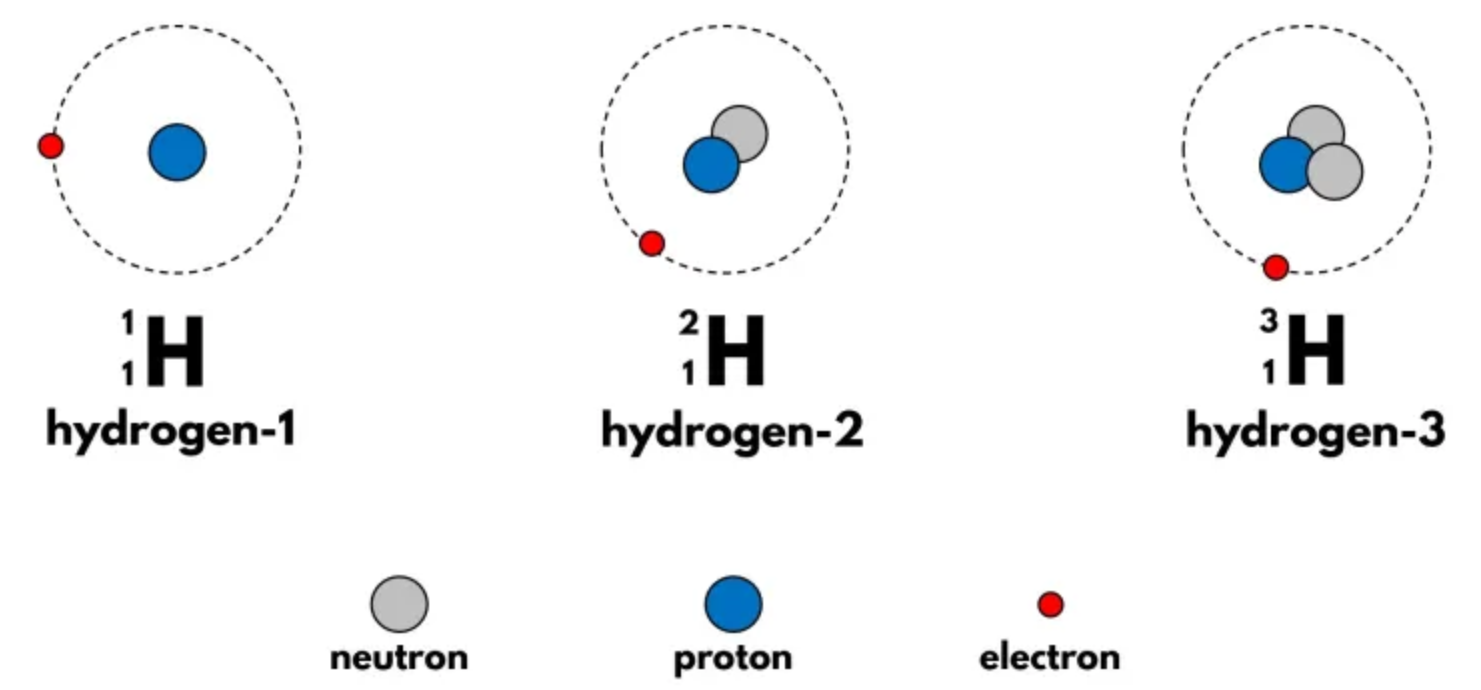
\includegraphics[width=0.75\linewidth]{hydro_iso}
  \end{center}

  \textbf{Applications}
  
  \begin{itemize}
  \item Semiconductor production enhancing Si-H bond by preventing
    chemical erosion and Hot Carrier Effect
  \item Chemical labeling to track chemical reactions
  \item Medicinal chemistry - FDA approved the first deuterium-labeled
    drug (\href{https://pubs.acs.org/doi/10.1021/acs.jmedchem.8b01808}{reference})
  \end{itemize}
\end{frame}

\begin{frame}{Experiment: Mass Spectroscopy}
  \begin{center}
    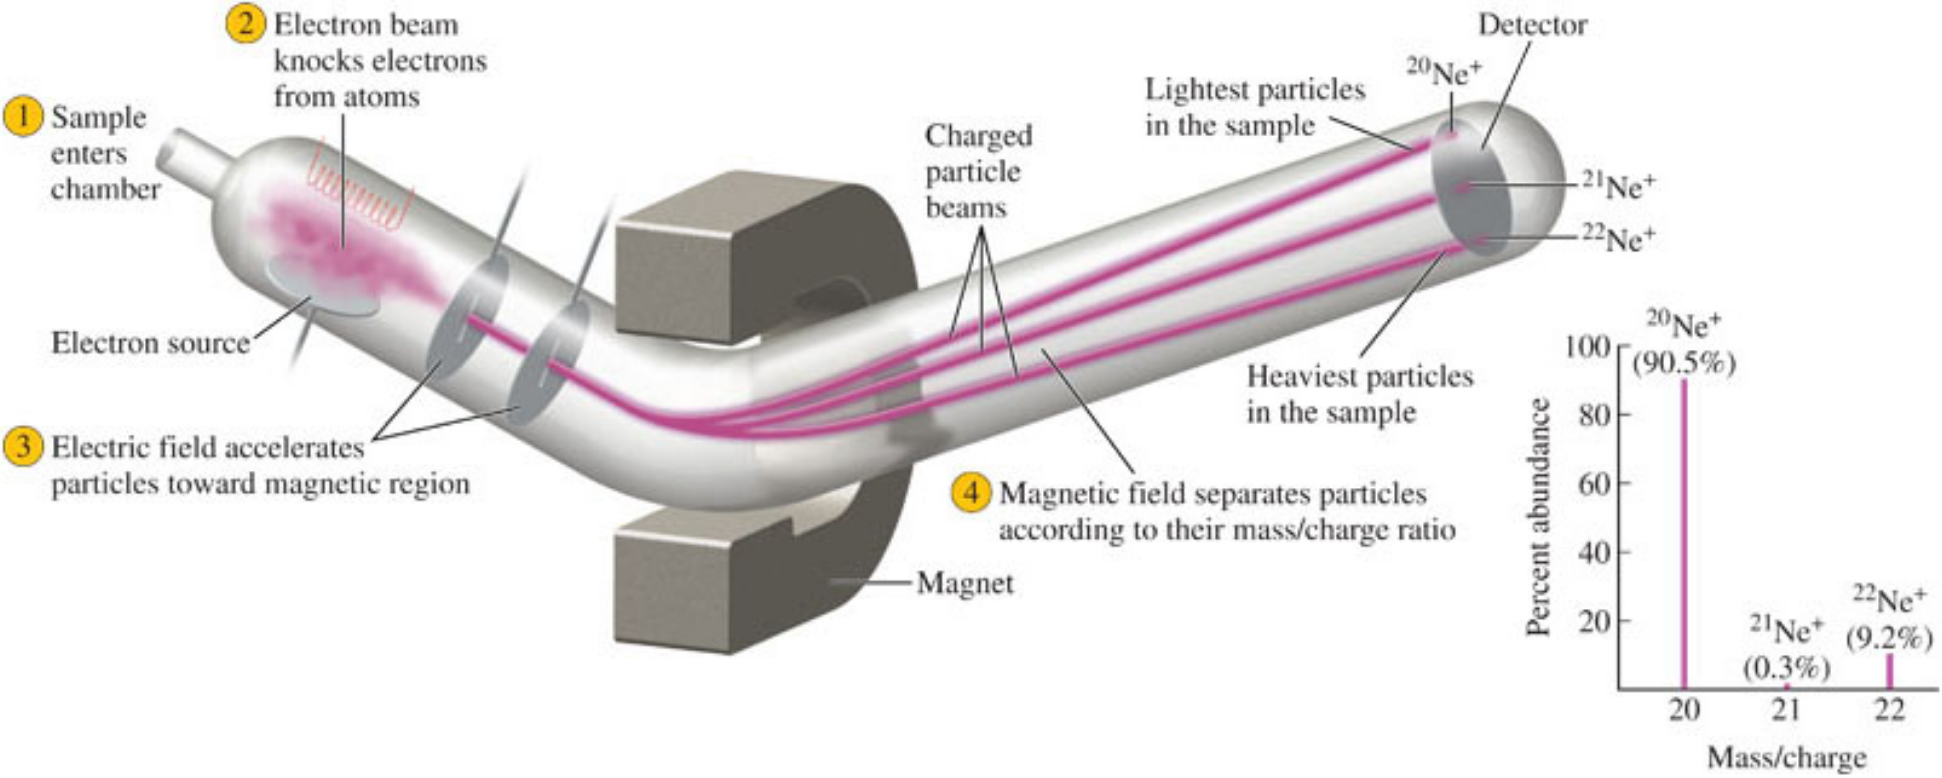
\includegraphics[width=\linewidth]{mass_spect}
  \end{center}

  \begin{itemize}
  \item Ionizes the atom and electric field accelerates atoms
  \item Time of flight - heavier atoms will travel slower
    than lighter ones
  \item Weighter average of atomic masses
  \end{itemize}  
\end{frame}

\section{Ionic and Molecular Compounds}

\begin{frame}{Ionic and Molecular Compounds}
  \textbf{Ionic Compounds}
  \begin{itemize}
  \item Consists of oppositely charged cations and anions
    such that the overall charge is neutral e.g CaCl$_2$(s),
    BaF(s), and Fe$_2$O$_3$(s)
  \item Electrolyte - substances that separate into the ions
    e.g. NaCl(aq) dissociates into Na$^+$ and Cl$^-$
  \item Forms ionic bonds (purely electrostatic interactions)
  \end{itemize}

  \textbf{Molecular Compounds}
  \begin{itemize}
  \item Composed of atoms from two or more nonmetals
  \item Forms covalent bonds (sharing of electrons)
  \end{itemize}
\end{frame}

\begin{frame}{Properties of Ionic and Molecular Compounds}
\end{frame}

\begin{frame}{Introduction to Bonding}
  \textbf{Ionic Bonding}
  \begin{itemize}
  \item Electrons transferred from metal
    to nonmetal
  \item Ionized atoms and electrostatic interactions
  \end{itemize}

  \textbf{Covalent Bonding (CB)}
  \begin{itemize}
  \item Sharing of electrons between atoms (usually
    look at as pairs)
  \item Generally occurs between nonmetals in molecular
    elements, molecular compounds, and polyatomic ions
  \end{itemize}
\end{frame}

\begin{frame}{CB: Consideration of Electronegativity}
\end{frame}

\subsection{Monatomic and Polyatomic Ions}

\begin{frame}{Monatomic and Polyatomic Ions}
\end{frame}

\subsection{Formulas for Ionic Compounds}

\begin{frame}{Molecular Formulas for Ionic Compounds}
\end{frame}

\section{Naming and Writing Formulas}

\subsection{Ionic Compounds}

\begin{frame}{Naming Ionic Compounds}
\end{frame}

\subsection{Molecular Compounds}

\begin{frame}{Naming Molecular Compounds}
\end{frame}

\subsection{Acids and Bases}

\begin{frame}{Definition of an Acid}
\end{frame}

\begin{frame}{Naming Acids and Bases}
\end{frame}

\end{document}
